\documentclass[12pt,a4paper]{report}
\usepackage[utf8]{inputenc}
\usepackage[english,russian]{babel}
\usepackage{indentfirst}
\usepackage{pdfpages}
\usepackage{titlesec}
\usepackage{listings}
\usepackage{amsmath}

\definecolor{friendlybg}{HTML}{f0f0f0}

% Вставка картинки
\usepackage{graphicx}
\graphicspath{{schemes/}}
\DeclareGraphicsExtensions{.pdf,.png,.jpg}

\usepackage[14pt]{extsizes}
%\usepackage{minted}

\newcommand{\hsp}{\hspace{20pt}}
\titleformat{\chapter}[hang]{\large\bfseries}{\thechapter{. }}{0pt}{\large\bfseries}
\titlelabel{hlabel-formati}
\titlespacing{\chapter}{42pt}{-20pt}{12pt}
\titleformat{\section}[hang]{\large\bfseries}{\thesection{. }}{0pt}{\large\bfseries}
\titlespacing{\section}{42pt}{12pt}{5pt plus 5pt}

\usepackage[tableposition=top,singlelinecheck=false]{caption}

% Отступ абзаца
\usepackage{indentfirst}
\setlength{\parindent}{1.5cm}

% Межстрочный интервал
\usepackage{setspace}
\onehalfspacing % интервал 1.5

\usepackage[left=3cm, right=1cm, top=2cm, bottom=2cm]{geometry}

%\renewcommand{\contentsname}{Содержание}

\AtBeginDocument{%
	\renewcommand\contentsname{Содержание}
}

\begin{document}
	
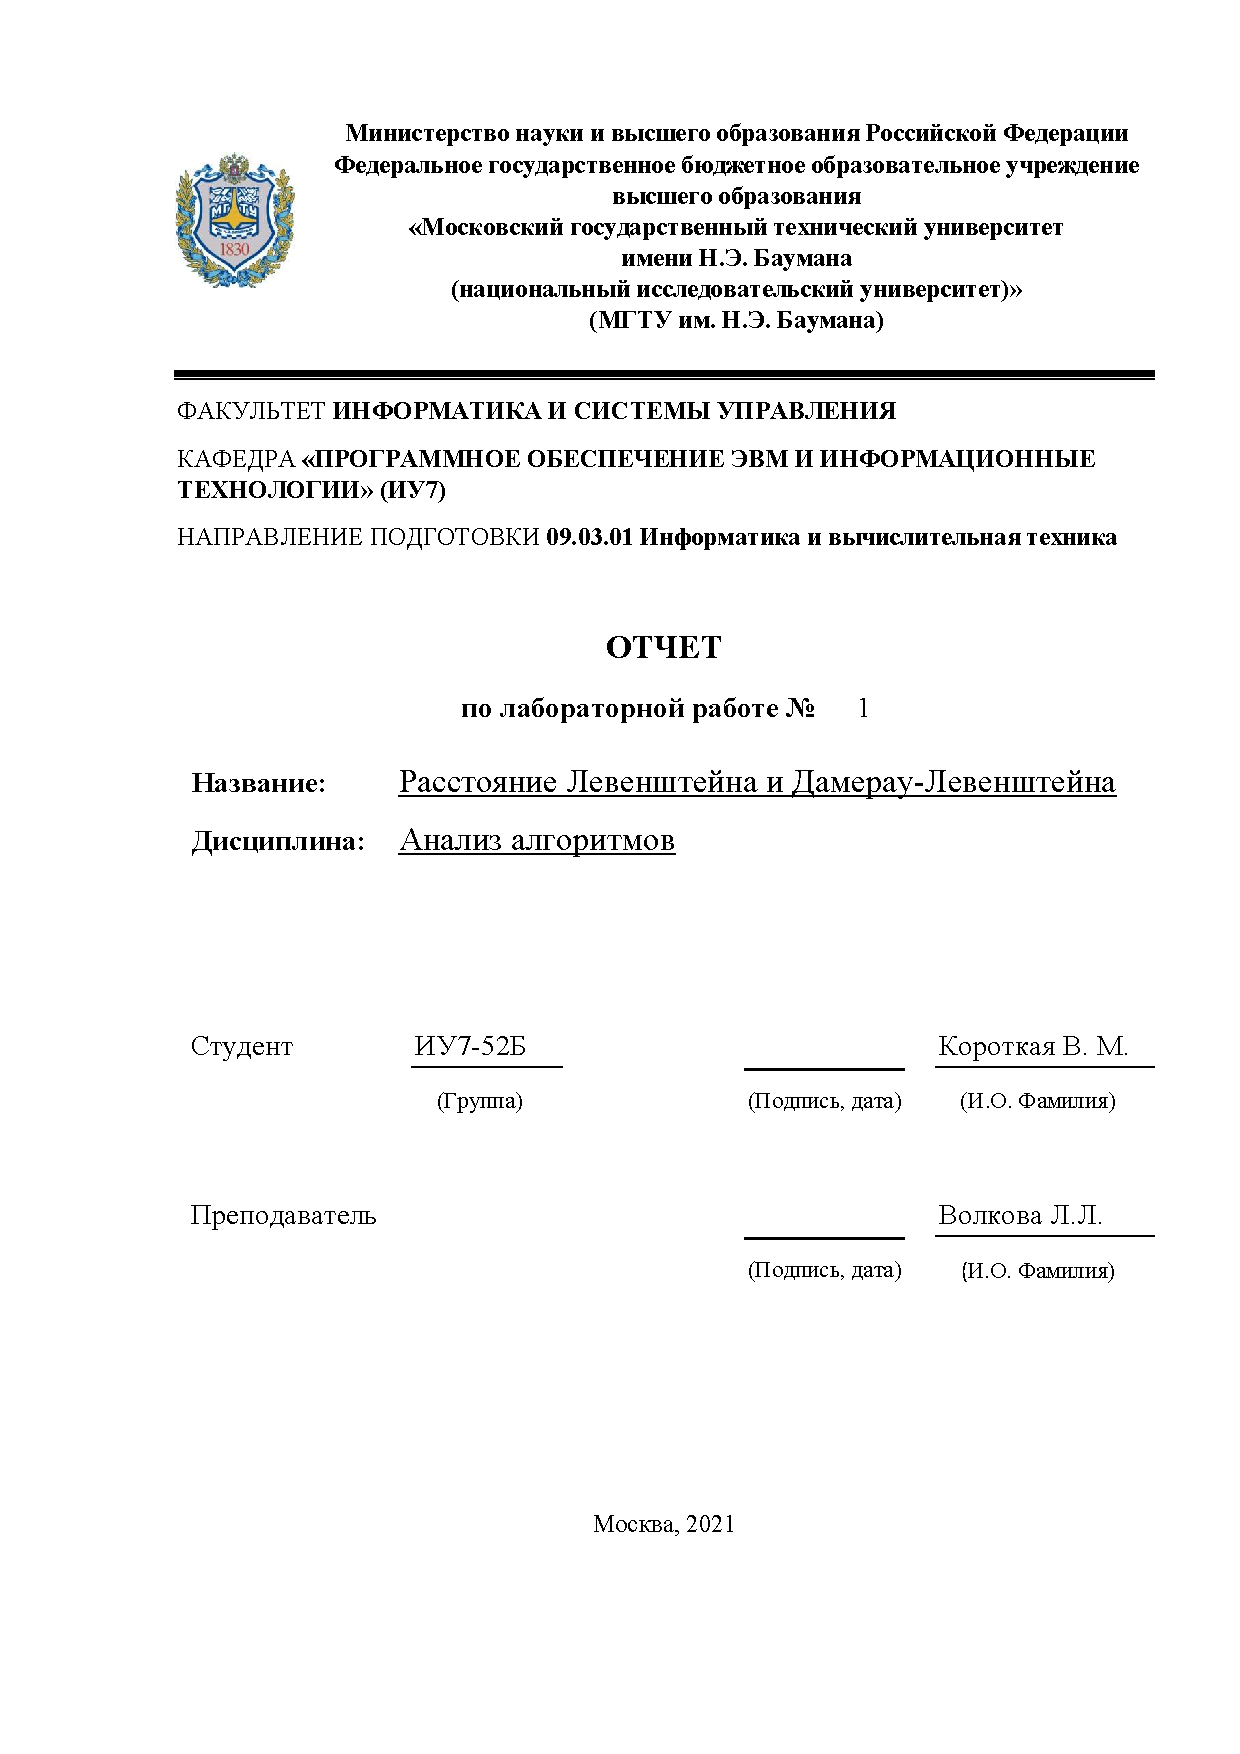
\includepdf[pages=1]{titul.pdf}

\tableofcontents{}

\newpage
\chapter*{Введение}
\addcontentsline{toc}{chapter}{Введение}

\textbf{Расстояние Левенштейна} (также известное как редакционное расстояние) 
в теории информации и компьютерной лингвистике – мера различия двух последовательностей символов 
(строк) относительно минимального количества операций вставки, удаления и замены, необходимых для
перевода одной строки в другую. Для одинаковых строк расстояние редактирования равно нулю. 

В 1965 году советский математик Владимир Иосифович Левенштейн разработал алгоритм, который позволяет 
оценить, насколько похожа одна строка на другую. Алгоритм Левенштейна дает возможность получить
именно численную оценку похожести строк.

Основная идея алгоритма состоит в том, чтобы посчитать 
минимальное количество операций удаления, вставки и замены, которые необходимо сделать над одной
из строк, чтобы получить вторую. 

В настоящее время алгоритм Левенштейна активно применяется в
различных программных продуктах, в том числе грамматических приложениях, таких как в MS Office
или подобных для решения следующих прикладных задач: 
\begin{itemize}
	\item в поисковых системах для нахождения объектов или записей по имени;
	\item в базах данных при поиске с неполно-заданным или неточно-заданным именем; 
	\item для исправления ошибок при вводе текста;
	\item для исправления ошибок в результате автоматического распознавания отсканированного текста или записей речи;
	\item в приложениях, связанных с автоматической обработкой текстов.
\end{itemize}

Функция Левенштейна может играть роль фильтра,
заведомо отбрасывающего неприемлемые варианты (у которых значение функции больше некоторой заданной константы).

Цель данной лабораторной работы заключается в реализации и последующем сравнении алгоритмов поиска 
расстояний Левенштейна и Дамерау-Левенштейна.\\

Для достижения поставленной цели необходимо выполнить следующие 
задачи:
\begin{itemize}
	\item математически описать расстояние Левенштейна и Домерау-Левенштейна;
	\item описать и реализовать алгоритмы поиска расстояний;
	\item замерить процессорное время работы алгоритмов при различных размерах строк;
	\item оценить наибольшую затрачиваемую память для каждого из алгоритмов;
	\item провести сравнительный анализ алгоритмов на основании проведённых экспериментов; 
\end{itemize}



\newpage
\chapter{Аналитическая часть}

В данном разделе будут рассмортенно формальное описание алгоритмов.

Поиск расстояний несёт в себе задачу нахождения такой последовательности операций, применение которых 
даст в результате минимальный суммарный штраф.

Существуют следующие штрафы:
\begin{itemize}
	\item вставка (I, от англ. insert) - 1;
	\item замена (R, от англ. replace) - 1;
	\item удаление (D, от англ. delete) - 1;
	\item совпадение (M, от англ. match) - 0;
	\item транспозиция (T, от англ. transposition) - 1.
\end{itemize}

Рассмотрим алгоритмы поиска расстояний Левенштейна и Дамерау-Левенштейна для строк \textit{S1} и \textit{S2} с длинами 
\textit{l1} и \textit{l2} соответственно.

\section{Расстояние Левенштейна, рекурсивный метод}

В методе используется рекурсивная формула нахождения \textit{ D(S1[1..i], S2[1..j])}, реализовать это можно 
с помощью рекурсивной функции. Функция будет принимать в качестве входных данных строки \textit{S1} и \textit{S2}, а 
также их длины \textit{i} и \textit{j} соответственно. Метод основан на последующем вызове той же функции для тех же 
строк, но для длин \textit{(i - 1, j - 1)}, \textit{(i - 1, j)}, \textit{(i, j - 1)}, где возвращается минимальное из этих значений. 

Данная проблема решается использованием рекуррентной формулы вычисления расстояний. Пусть \textit{D(S1[1..i]}, 
\textit{S2[1..j])} - расстояние Левенштейна для подстроки \textit{S1} и \textit{S2} с длинами \textit{i} и \textit{j} соответственно.\

Тогда, формула для вычисления \textit{D} имеет следующий вид:

\begin{displaymath}
	D(i,j) = \left\{ 
	\begin{array}{ll}
		j, & \textrm{если i = 0} \\
		i, & \textrm{если j = 0} \\
		min(D(S1[1..i], S2[1..j-1]) + 1,\\
		D(S1[1..i-1], S2[1..j]) + 1,\\
		D(S1[1..i-1], S2[1..j-1] + \left \{ 
		\begin{array}{ll}
			0, \textrm{если S1[i] = S2[j]} \\ 
			1, \textrm{иначе}
		\end{array} \right.
		)
	\end{array} \right.
\end{displaymath} \\

\section{Расстояние Левенштейна, матричный метод}

Данный матричный метод основан на использовании рекуррентной формулы. В начале работы создаётся 
целочисленная матрица с размерами \textit{(l1 + 1)} на \textit{(l2 + 1)}, затем заполняются первый столбец и первая 
строка, которые являются базой для рекуррентной формулы. Матрица заполняется построчно, в каждой 
ячейке \textit{[i][j]} матрицы записывается значение \textit{D(S1[1..i - 1], S2[1..j - 1])}. В том случае, когда \textit{i = 1} и 
\textit{j = 1} будет значить, что строки пусты. Итоговым результатом является значение в нижней правой ячейке
матрицы, т.е. в ячейке с индексом \textit{[l1 + 1][l2 + 1]}. 

\section{Расстояние Левенштейна, рекурсивный метод с заполнением матрицы}

В данном методе создаётся матрица размерами \textit{(l1 + 1)} на \textit{(l2 + 1)}, все ячеки которой изначально заполнены 
значением бесконечности. В каждой клетке \textit{[i][j]} этой матрицы будет записано значение \textit{D(s1[1..i - 1], s2[1..j - 1])}.

Рекурсивная функция получает матрицу, индексы \textit{i}, \textit{j} положения в ней и две строки. Алгоритм начинает свою 
работу с ячейки \textit{[1][1]}, которая заполняется значением \textit{0}. Из положения \textit{[i][j]} рассматривается переход в 
соседние ячейки \textit{[i + 1][j + 1], [i + 1][j], [i][j + 1]}. В случае, если соседняя ячейка расположена в 
пределах матрицы и расстояние R при переходе из данной ячейки меньше ныне хранимого в ней значения, то 
значение соседней ячейки меняется на R, после чего функция запускается уже для соседней ячейки. После 
завершения работы всех функций, расстояние Левенштейна расположено в ячейке \textit{[l1 + 1][l2 + 1]}. 

\section{Расстояние Дамерау-Левенштейна, матричный метод}


Метод является модифицированным методом подсчёта расстояния Левенштейна матричным методом. В матрице
для ячейки \textit{[i][j]}, где \textit{i > 2} и \textit{j > 2}, учитывается также вариант перехода из клетки \textit{[i - 2][j - 2]}, в 
случае когда \textit{S1[i] = S2[j-1]} и \textit{S1[i-1] = S[j]}. Результатом всё также будет правое нижнее значение
ячейки \textit{[l1 + 1][l2 + 1]}. 

Аналогично и для Дамерау-Левенштейна:

\begin{displaymath}
	D(i, j) = \left\{
	\begin{array}{ll}
		j, \textrm{если i = 0} \\
		i, \textrm{если j = 0} \\
		min(D(S1[1..i], S2[1..j-1]) + 1,\\
		D(S1[1..i-1], S2[1..j]) + 1,\\
		D(S1[1..i-1], S2[1..j-1] + \left \{ 
		\begin{array}{ll}
			0, \textrm{если S1[i] = S2[j]} \\ 
			1, \textrm{иначе}
		\end{array} \right.
		, \\
		\left \{ \begin{array}{ll}
			D(S1[1..i-2], S2[1..j-2]) + 1 \textrm{, если} \left \{ 
			\begin{array}{ll}
				i > 1, j > 1 \\
				S1[i] = S2[j-1] \\
				S1[i-1] = S2[j]
			\end{array} \right. \\
			+\infty, \textrm{иначе}
		\end{array} \right. 
		)
	\end{array} \right.
\end{displaymath}

\section*{Вывод}

В данном раздели были рассмотрены алгоритмы нахождения расстояния Левенштейна и Дамерау-Левенштейна, который является модификацией первого (учитывает возможность перестановки соседних символов).

Входными данными реализуемого ПО являются две символьные строки.

Выходными данными реализуемого ПО являеться результат алгоритмов поиска расстояний т. е.:
\begin{itemize}
	\item число (результат) - для Рекурсивной реализации Левенштейна;
	\item число (результат) и матрица расстояний - для Матричной реализации Левенштейна;
	\item число (результат) и матрица расстояний - для Матричной-Рекурсивной реализации Левенштейна;
	\item число (результат) и матрица расстояний - для Матричной реализации Дамерау-Левенштейна;
\end{itemize}

Ограничением для реализуемого ПО является - ввод двух символьный строк, каждой с новой строки.



\newpage
\chapter{Конструкторская часть}

В данном разделе представлены схемы алгоритмов. Так же будут описаны пользовательские структуры данных, приведены структура ПО и классы эквивалентности для тестирования реализуемого ПО.

\section{Схемы алгоритмов}

\section*{Расстояние Левенштейна, рекурсивный метод}

\begin{figure}[ht]
	\center{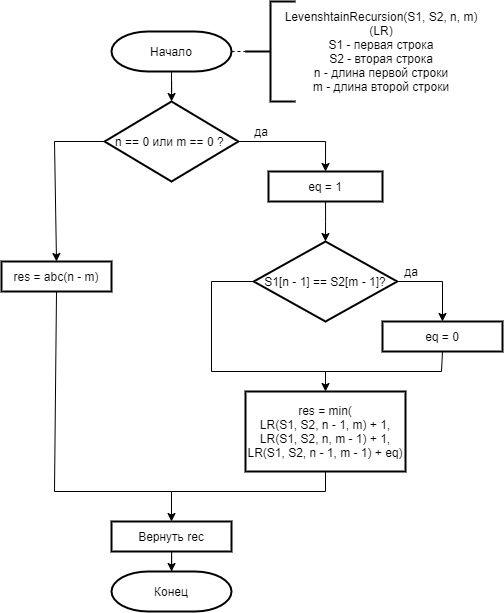
\includegraphics[scale=0.6]{levRec}}
	\caption{Рекурсивный алгоритм Левенштейна}
	%\label{fig:image}
\end{figure}

\newpage
\section*{Расстояние Левенштейна, матричный метод} \

\begin{figure}[ht]
	\center{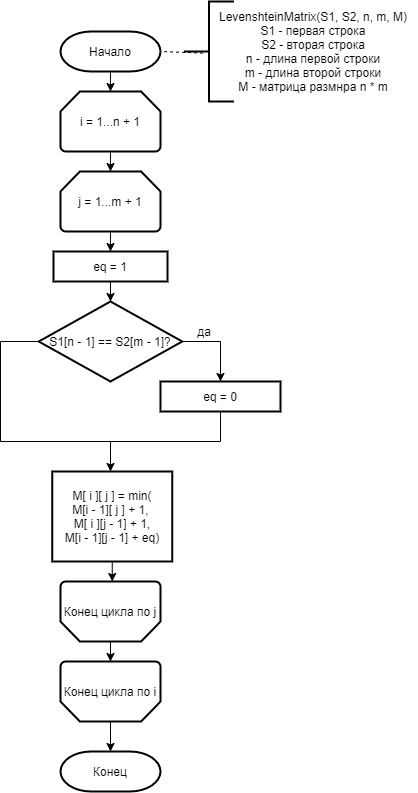
\includegraphics[scale=0.6]{levMat}}
	\caption{Матричный алгоритм Левенштейна}
	%\label{fig:image}
\end{figure}

\newpage
\section*{Расстояние Левенштейна, рекурсивный метод с заполнением матрицы}
\begin{figure}[ht]
	\center{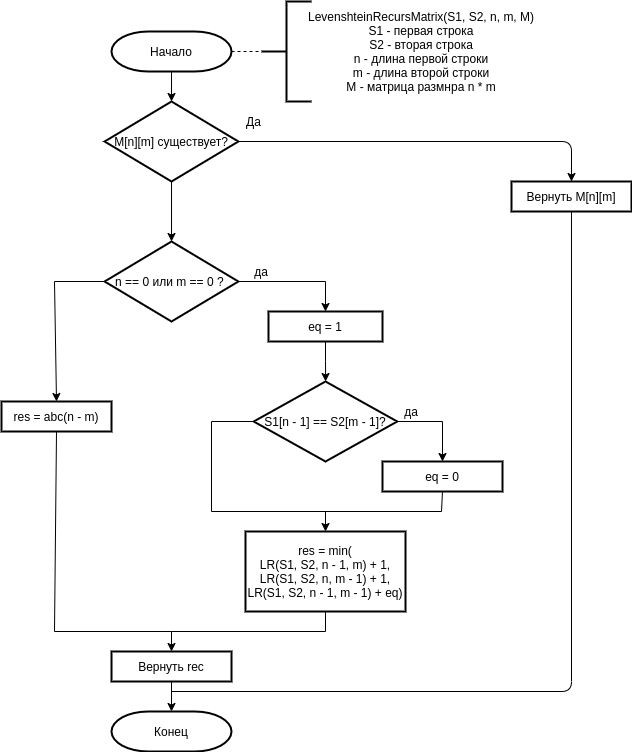
\includegraphics[scale=0.59]{levRecMat}}
	\caption{Рекурсивный алгоритм Левенштейна, с заполнением матрицы}
	%\label{fig:image}
\end{figure}


\newpage
\section*{Расстояние Дамерау-Левенштейна, матричный}
\begin{figure}[ht]
	\center{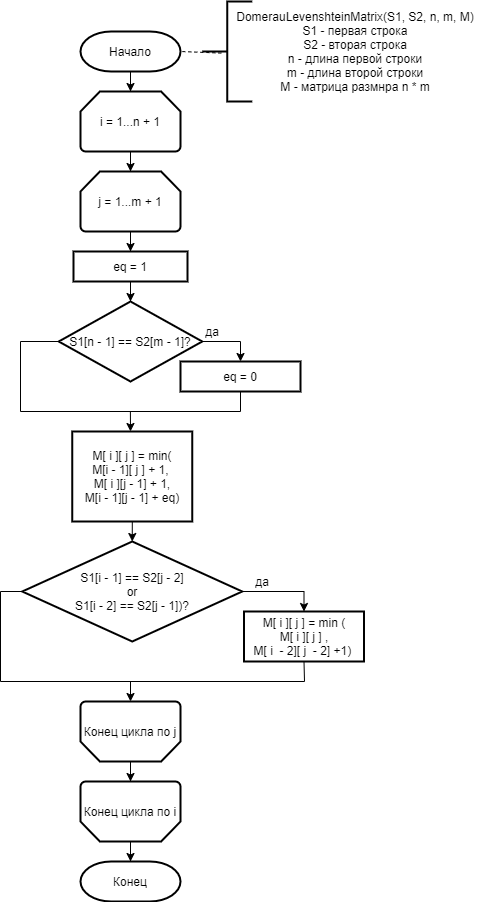
\includegraphics[scale=0.59]{domLevMat}}
	\caption{Матричный алгоритм Дамерау-Левенштейна}
	%\label{fig:image}
\end{figure}

\newpage
\section{Структура ПО}

На рисунке 2.5 представлена диограмма классов.

\section*{}
\begin{figure}[ht]
	\center{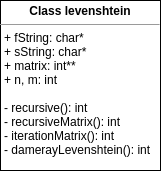
\includegraphics[scale=0.8]{structPO}}
	\caption{Диаграмма классов реализуемого ПО}
	%\label{fig:image}
\end{figure}

\section{Тестирование}

В рамках данной лабораторной работы были выделены следующие классы эквивалентности:
\begin{itemize}
	\item входными данными являются две одинаковые строки;
	\item входными данными являються пустые строки;
	\item входными данными являються строки содержавшие одинаковые последовательно символы в разном регистре;
	\item входными данными являються строки без совподающих символов.
\end{itemize}

Для проверки работы программы будет осуществлено тестирование согласно классам эквивалентности.

\section*{Вывод}

В данном разделе были построены схемы алгоритмов, выделены классы эквивалентности и создана диаграмма классов.

\newpage
\chapter{Технологическая часть} 

В данном разделе приведены средства реализации, требования к ПО и листинги кода.

\section{Средства реализации}
В качестве языка программирования был выбран с++. Данный язык знаком и предостовляет все необходимые ресурсы.
В качестве среды разработки я использовала Visual Studio Code, т.к. считаю его достаточно удобным и легким.
Visual Studio Code подходит не только для  Windows, но и для Linux, это еще одна причина, по которой я выбрала VS code, т.к. у меня установлена ОС  fedora 34.

\section{Требования к ПО}

К программе предъявляется требования:

\begin{itemize}
	\item на вход подаются две строки;
	\item на выходе - искомое расстояние для четырех методов.
\end{itemize} 


\section{Сведения о модулях программы}

Данная программа разбита на модули:

\begin{itemize}
	\item main.cpp - Файл, содержащий точку входа в программу. В нем происходит общение с пользователем и вызов алгоритмов;
	\item levenshtain.cpp - Файл содержит непосредственно сами алгоритмы;
\end{itemize}

\section{Листинг кода}

\noindent\textrm{Листинг 3.1: Левенштейна, рекурсивный метод}
\begin{lstlisting}[frame=single, numbers=left]	
int Levenshtein::recursive()
{	
	int i = n;
	int j = m;
	return getDistance(i, j);
}

int Levenshtein::getDistance(int i, int j)
{
	if (!i)
		return j;
	if (!j)
		return i;
	flag = 1;
	if (fString[i - 1] == sString[j - 1])
		flag = 0;
	return min(min(getDistance(i, j - 1) + 1,
		getDistance(i - 1, j) + 1),
			getDistance(i - 1, j - 1) + flag);
}
\end{lstlisting}



\noindent\textrm{Листинг 3.2: Левенштейна, матричный метод}
\begin{lstlisting}[frame=single, numbers=left]
int Levenshtein::iterativeMatrix()
{
	resetMatrix();
	for (int i = 1; i < n + 1; i++)
	{
		for (int j = 1; j < m + 1; j++)
	{
		if (fString[i - 1] == sString[j - 1])
			flag = 0;
		else
			flag = 1;
		matrix[i][j] = min(matrix[i - 1][j] + 1,
			min(matrix[i][j - 1] + 1,
			matrix[i - 1][j - 1] + flag));
	}
	}
	outputMatrix();
	return matrix[n][m];
}
\end{lstlisting}




\noindent\textrm{Листинг 3.3: Левенштейна, рекурсивный метод с заполнением матрицы}
\begin{lstlisting}[frame=single, numbers=left]
int Levenshtein::recursiveMatrix()
{
	resetMatrix();
	int i = n;
	int j = m;
	getDistanceRec(i, j);
		
	outputMatrix();
	return matrix[n][m];
}
	
int Levenshtein::getDistanceRec(int i, int j)
{
	if (matrix[i][j] != -1)
	return matrix[i][j];
	if (!i)
	{
		matrix[i][j] = j;
		return matrix[i][j];
	}
	if (!j)
	{
		matrix[i][j] = i;
		return matrix[i][j];
	}
	flag = 1;
	if (fString[i - 1] == sString[j - 1])
		flag = 0;
	matrix[i][j] = min(min(getDistance(i, j - 1) + 1, 
		getDistance(i - 1, j) + 1),
		getDistance(i - 1, j - 1) + flag);
		return matrix[i][j];
}
\end{lstlisting}



\noindent\textrm{Листинг 3.4: Дамерау-Левенштейна, матричный метод}
\begin{lstlisting}[frame=single, numbers=left]
int Levenshtein::damerauLevenshtein()
{
	resetMatrix();
	for (int i = 1; i < n + 1; i++)
	{
	  for (int j = 1; j < m + 1; j++)
      {
    	if (fString[i - 1] == sString[j - 1])
			flag = 0;
		  else
			flag = 1;
		matrix[i][j] = min(matrix[i - 1][j] + 1, 
			min(matrix[i][j - 1] + 1, 
			matrix[i - 1][j - 1] + flag));
			
		if ((i > 1) && (j > 1)  && 
		  ((fString[i - 1] == sString[j - 2]) ||
		   (fString[i - 2] == sString[j - 1])))
		  
		  matrix[i][j] = min(matrix[i][j], 
				matrix[i - 2][j - 2] + 1);
	  }
	}
	outputMatrix();
	return matrix[n][m];
}
\end{lstlisting}

\newpage
\section{Тестирование}

%В данном разделе будет приведена таблица \ref{table:ref1}, в которой четко отражено тестирование программы. Первый и второй столбец отвечают за введенные пользователем слова.\\

\begin{table}[ht!]
	\centering
	\caption{Таблица тестов}
	\label{table:ref1}
	\begin{tabular}{ | l | l | l | l |}
		\hline
		Слово 1 & Слово 2 & Ожидаемый вывод &  Вывод программы  \\ \hline
		сито & столб & 3 & 3 \\ \hline
		exponential & polynomial & 6 & 6 \\ \hline
		Vera & Vera & 0 & 0 \\ \hline
		Vera & vera & 1 & 1 \\ \hline
		ma  & am & 2 1 &  2 1 \\ \hline
		& & 0 & 0 \\ \hline
		abc & cab & 2 & 2 \\ \hline
		\hline
	\end{tabular}
\end{table} 


Все тесты пройдены успешно.

\section{Вывод}

В данном разделе были рассмотрены листинги кода, обоснован выбор использованного в данной работе языка программирования и среды разработки, а также была произведена проверка корректной работы программы, благодаря таблице \ref{table:ref1}.
Сравнив представленные листинги, можно сказать, что написание рекуррентных подпрограмм проще, чем матричных.

\newpage
\chapter{Исследовательская часть}

В данном разделе сравним работу каждого алгоритма.

\section{Временные характеристики}

Сравним матричный алгоритм Левенштейна и Дамерау-Левенштейна. Для сравнения возьмем 
строки длинной [10, 20, 30, 50, 100, 200]. Воспользуемся усреднением массогово эксперимента.
Для этого сложим результат работы n экспериментов(n >= 10). После чего поделим на n.
Возьмем n = 500. Резултат можно увидеть на рисунке  . При короткой длинне строк разница почти
не заметна, но при увелечении длины Дамерау-Левенштен уступает Левенштейну в силу дополнительной операции в Дамерау-Левенштейне.

\begin{figure}[ht!]
	\centering{
		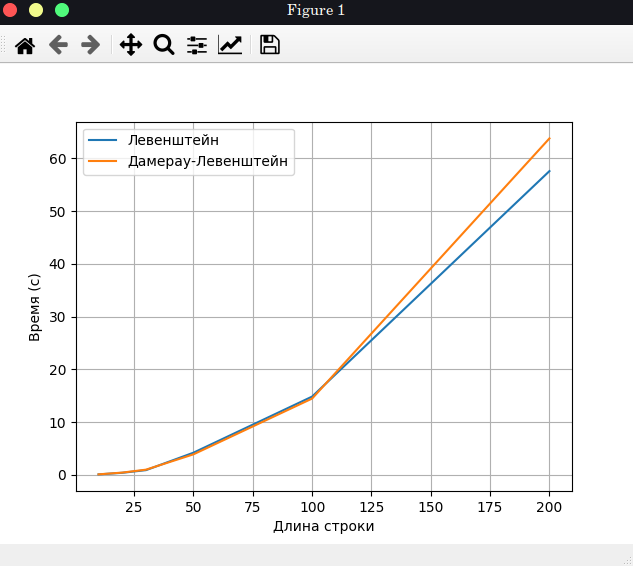
\includegraphics[width=0.6\textwidth]{graphLev-LevDam.png}
		\caption{Сравнение времени работы алгоритма поиска расстояния Левенштейна и Дамерау-Левенштейна}
		\label{fg:ref4}}
\end{figure}

Далее проведем сравнительный анализ рекурсеонного и матричного Левенштейна. Вольмем строки длинной [2, 3, 4, 5, 6, 7], при n = 50. Результат на рисунке  .Рост времени выполнения рекурсии обусловлен повторными вызовами с однотипнами параметрами. 

\begin{figure}[ht!]
	\centering{
		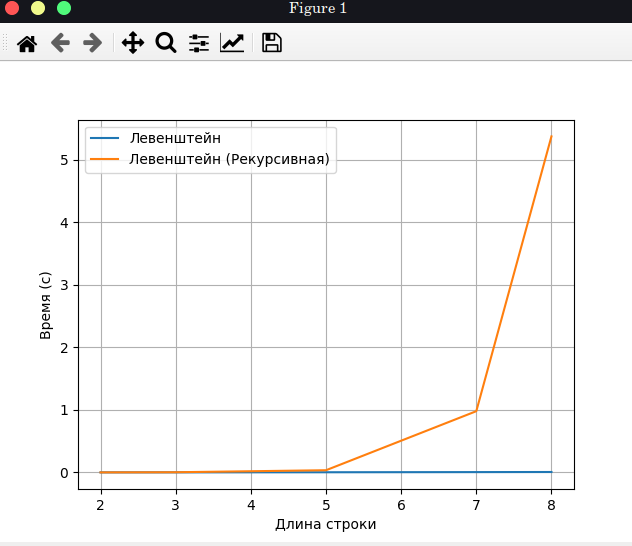
\includegraphics[width=0.6\textwidth]{graphLev-LevRec.png}
		\caption{Сравнение времени работы рекурсивной и матричной реализаций алгоритма Левенштейна.}
		\label{fg:ref5}}
\end{figure}

\section{Характеристики по памяти}

На рисунке  представлено дерево вызовов рекурсивного алгоритма Левенштейна.
Видно, что на третьем уровне встречаются повторные вызовы. 
Чем больше будет уровень, тем чаще будут вызываться функции с однотипными аргументами, что может привести к превышению максимальной глубины рекурсии. 
При строках длиной 2 подпрограмма вызовется 18 раз. 
Каждый вызов задействует 32 мегабайт (замеры проведены с помощью  библиотеки memory\_profiler ).
В итоге нам потребуется 576 мегабайт для рекурсивных вызовов, в то время, когда в матричном алгоритме используется 42 мегабайта. 


\begin{figure}[ht!]
	\centering{
		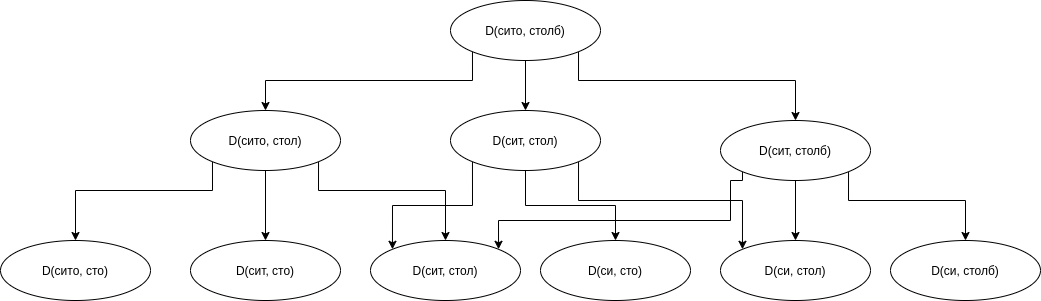
\includegraphics[width=0.8\textwidth]{rec_example.png}
		\caption{Сравнение времени работы рекурсивной и матричной реализаций алгоритма Левенштейна.}
		\label{fg:ref6}}
\end{figure}

\section{Сравнительный анализ алгоритмов}

Приведенные характеристики показывают нам, что рекурсивная реализация алгоритма очень сильно проигрывает по времени и по памяти.\\
Во время печати очень часто возникают ошибки связанные с транспозицией букв, поэтому алгоритм поиска расстояния Дамерау-Левенштейна предпочтительнее, не смотря на то, что он проигрывает по времени алгоритму Левенштейна.\\
По аналогии с первым абзацем можно сделать вывод о том, что рекуррентный алгоритм поиска расстояния Дамерау-Левенштейна будет более затратный, как по памяти, так и по времени по сравнению с матричной реализацией алгоритма поиска расстояния Дамерау-Левенштейна.


\section{Вывод}

В данном разделе было произведено сравнение количества затраченного времени и памяти вышеизложенных алгоритмов.
Самым быстрым оказался матричный алгоритм нахождения расстояния Левенштейна.

\newpage
\chapter*{Заключение}
\addcontentsline{toc}{chapter}{Заключение}

Алгоритмы поиска расстояний Левенштейна и ДамерауЛевенштейна являются самыми популярными алгоритмами, которые помогают найти редакторское расстояние. \\
В этой лабораторной работе мы познакомились с алгоритмами поиска расстояний Левенштейна (Формула \ref{eq:ref1}) и Дамерау-Левенштейна (Формула \ref{eq:ref2}).
Построили схемы (Рисунок \ref{fg:ref1}, Рисунок \ref{fg:ref2}), соответствующие данным алгоритмам, также разобрали рекуррентные реализации (Рисунок \ref{fg:ref3}).
Написали полностью готовый и протестированный (Таблица \ref{table:ref1}) программный продукт, который считает дистанцию 4 способами.



В рамках выполнения работы решены следующие задачи.

\begin{enumerate}
	\item Изучены алгоритмы поиска расстояний Дамерау-Левенштейна и Левенштейна.
	\item Реализованы изученные алгоритмы, а также матричную и рекурсивную реализации алгоритма.
	\item Проиллюстрированы алгоритмы схемами.
	%	\item Описали выбранную среду разработки и ЯП.
	\item Проведено сравнение временных характеристик, а также затраченной памяти.
\end{enumerate}


\newpage
\renewcommand\bibname{Список литературы}
\addcontentsline{toc}{chapter}{Список литературы}
\makeatletter % список литературы
\def\@biblabel#1{#1. }
\makeatother
\begin{thebibliography}{2}
	\bibitem{analyse_info} Дж. Макконнел. Анализ алгоритмов. Активный обучающий подход. -- М.: Техносфера, 2017. -- 267с.
	\bibitem{analyse_info} Карахтанов, Д. С. Программная реализация алгоритма Левенштейна для устранения опечаток в записях баз данных
	/ Д. С. Карахтанов. — Текст : непосредственный // Молодой ученый. — 2010. — № 8 (19). — Т. 1. — С. 158-162. — 
	URL: https://moluch.ru/archive/19/1966/ (дата обращения: 24.10.2021).
	\bibitem{analyse_info}В. И. Левенштейн. Двоичные коды с исправлением выпадений, вставок и замещений символов. Доклады Академий Наук СССР, 1965. 163.4:845-848.
	\bibitem{anatyse_info}Основы программирования на языках Си и C++ для начинающих[Электронный ресурс]. Режим доступа: http://cppstudio.com/ (дата обращения 10.10.2021)
	\bibitem{analyse_info}LINUX.ORG.RU - Русскоязычная информация о ОС Linux[Электронный ресурс] Режим доступа://www.linux.org.ru/(дата обращения 25.10.2021)
	
	%\bibitem{time_bib} Документация на официальном сайте Python про библиотеку time [Электронный ресурс]. Режим доступа: https://docs.python.org/3/library/time.html (дата обращения 23.09.2020)
\end{thebibliography}

\end{document}